\chapter{Figures}
\label{cha:app_figures}

\redtxt{figures que sobren}

\section{Figures of disconnected meanings for the \secondmodel{}}
\label{sec:app_figures_second-model}

Section \ref{sec:results_new_other} shows the results obtained for the current model.
For comparison with \cite{Ferrer2003a}, figures generated from the same sets of parameters as for Figures \ref{fig:informationTheoretic_uniform_phi0_nm400_dynamic_randomBipartite_allowUnlinked},  \ref{fig:informationTheoretic_uniform_phi0_nm400_dynamic_singleLink_allowUnlinked} and \ref{fig:informationTheoretic_uniform_phi0_nm400_dynamic_oneToOne_allowUnlinked} but with disconnected meanings kept disallowed are shown as Figures \ref{fig:informationTheoretic_uniform_phi0_nm400_dynamic_randomBipartite_disallowUnlinked},  \ref{fig:informationTheoretic_uniform_phi0_nm400_dynamic_singleLink_disallowUnlinked} and \ref{fig:informationTheoretic_uniform_phi0_nm400_dynamic_oneToOne_disallowUnlinked} respectively.
Statistical measures for chosen values of $\lambda$ are shown in Figures \ref{fig:insideLambda_uniform_phi0_nm400_dynamic_randomBipartite_disallowUnlinked}, \ref{fig:insideLambda_uniform_phi0_nm400_dynamic_singleLink_disallowUnlinked} and \ref{fig:insideLambda_uniform_phi0_nm400_dynamic_oneToOne_disallowUnlinked}.

\begin{figure}
  \centering
  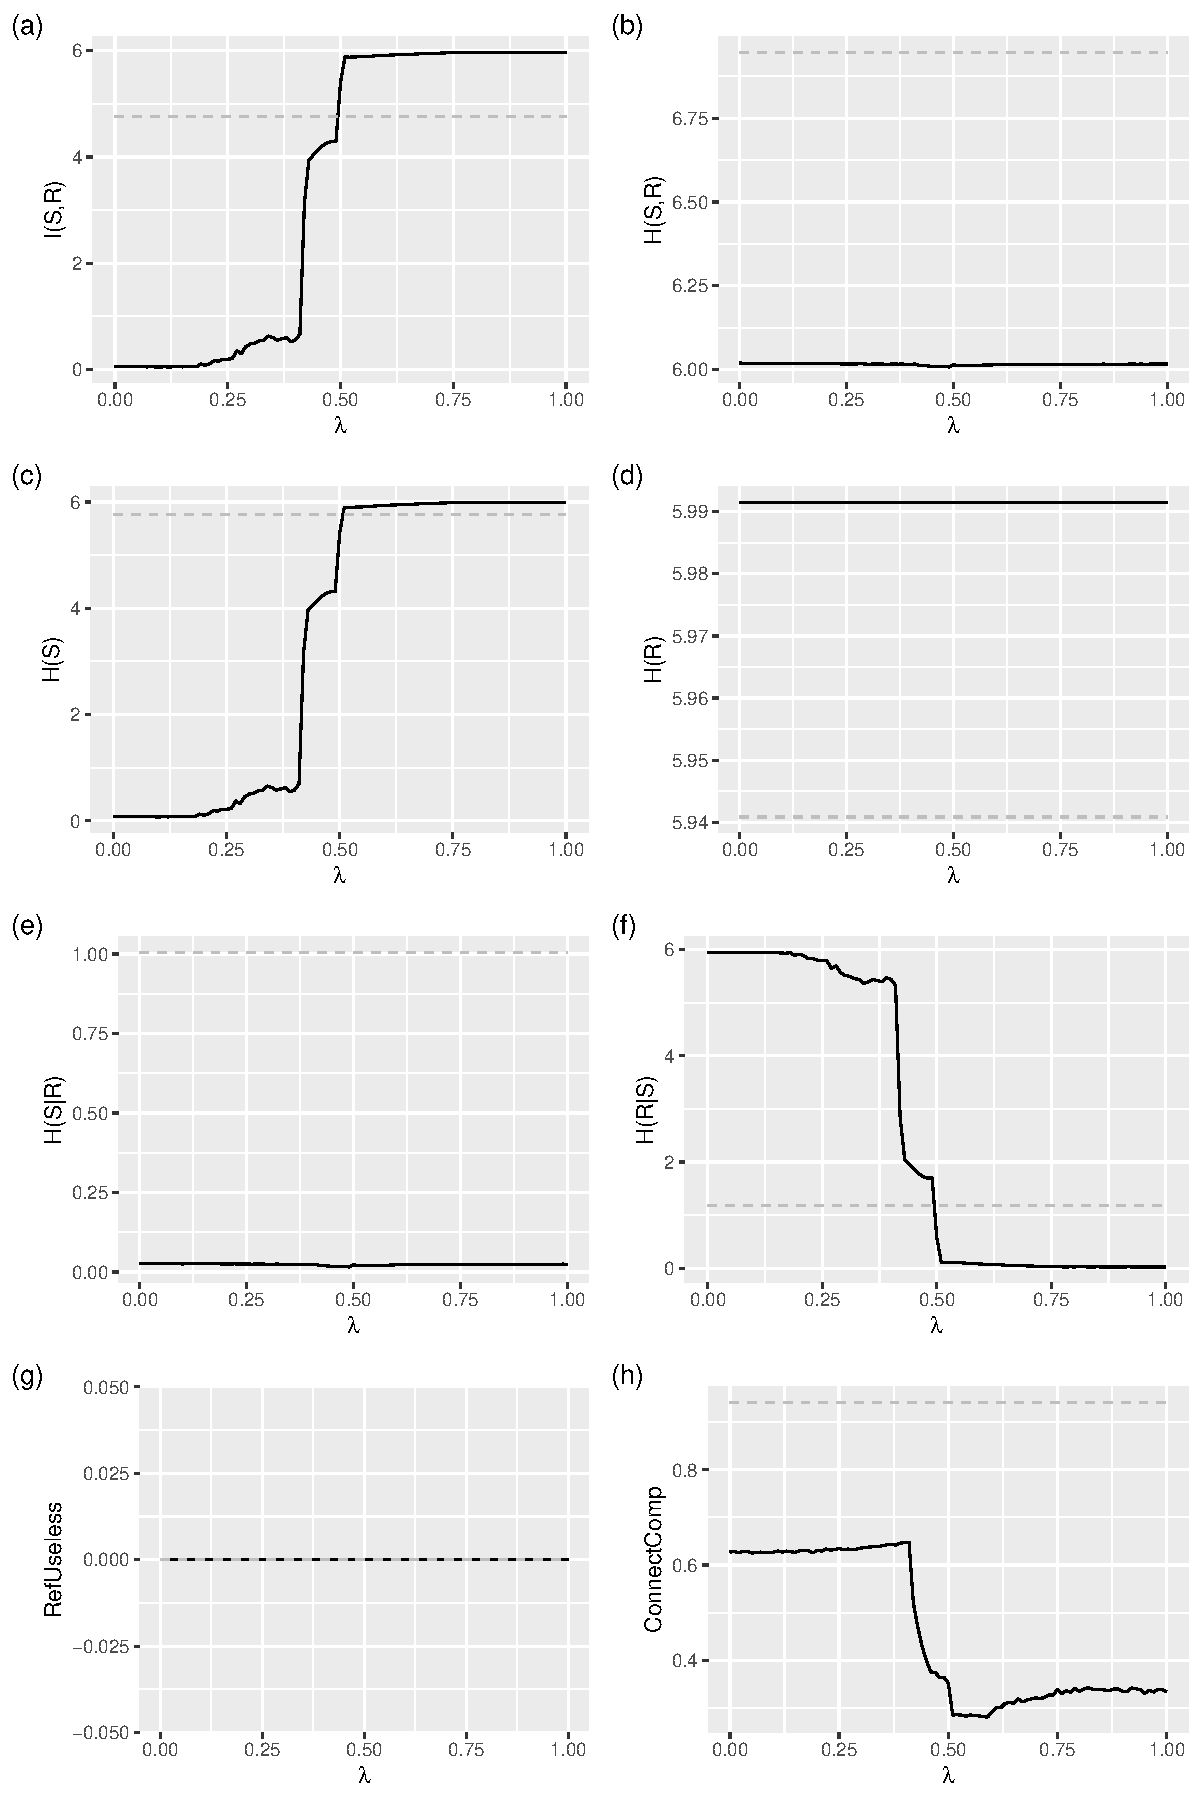
\includegraphics[width=\textwidth]{informationTheoretic_uniform_phi0_nm400_dynamic_randomBipartite_disallowUnlinked}
  \caption{a}
  \label{fig:informationTheoretic_uniform_phi0_nm400_dynamic_randomBipartite_disallowUnlinked}
\end{figure}

\begin{figure}
  \centering
  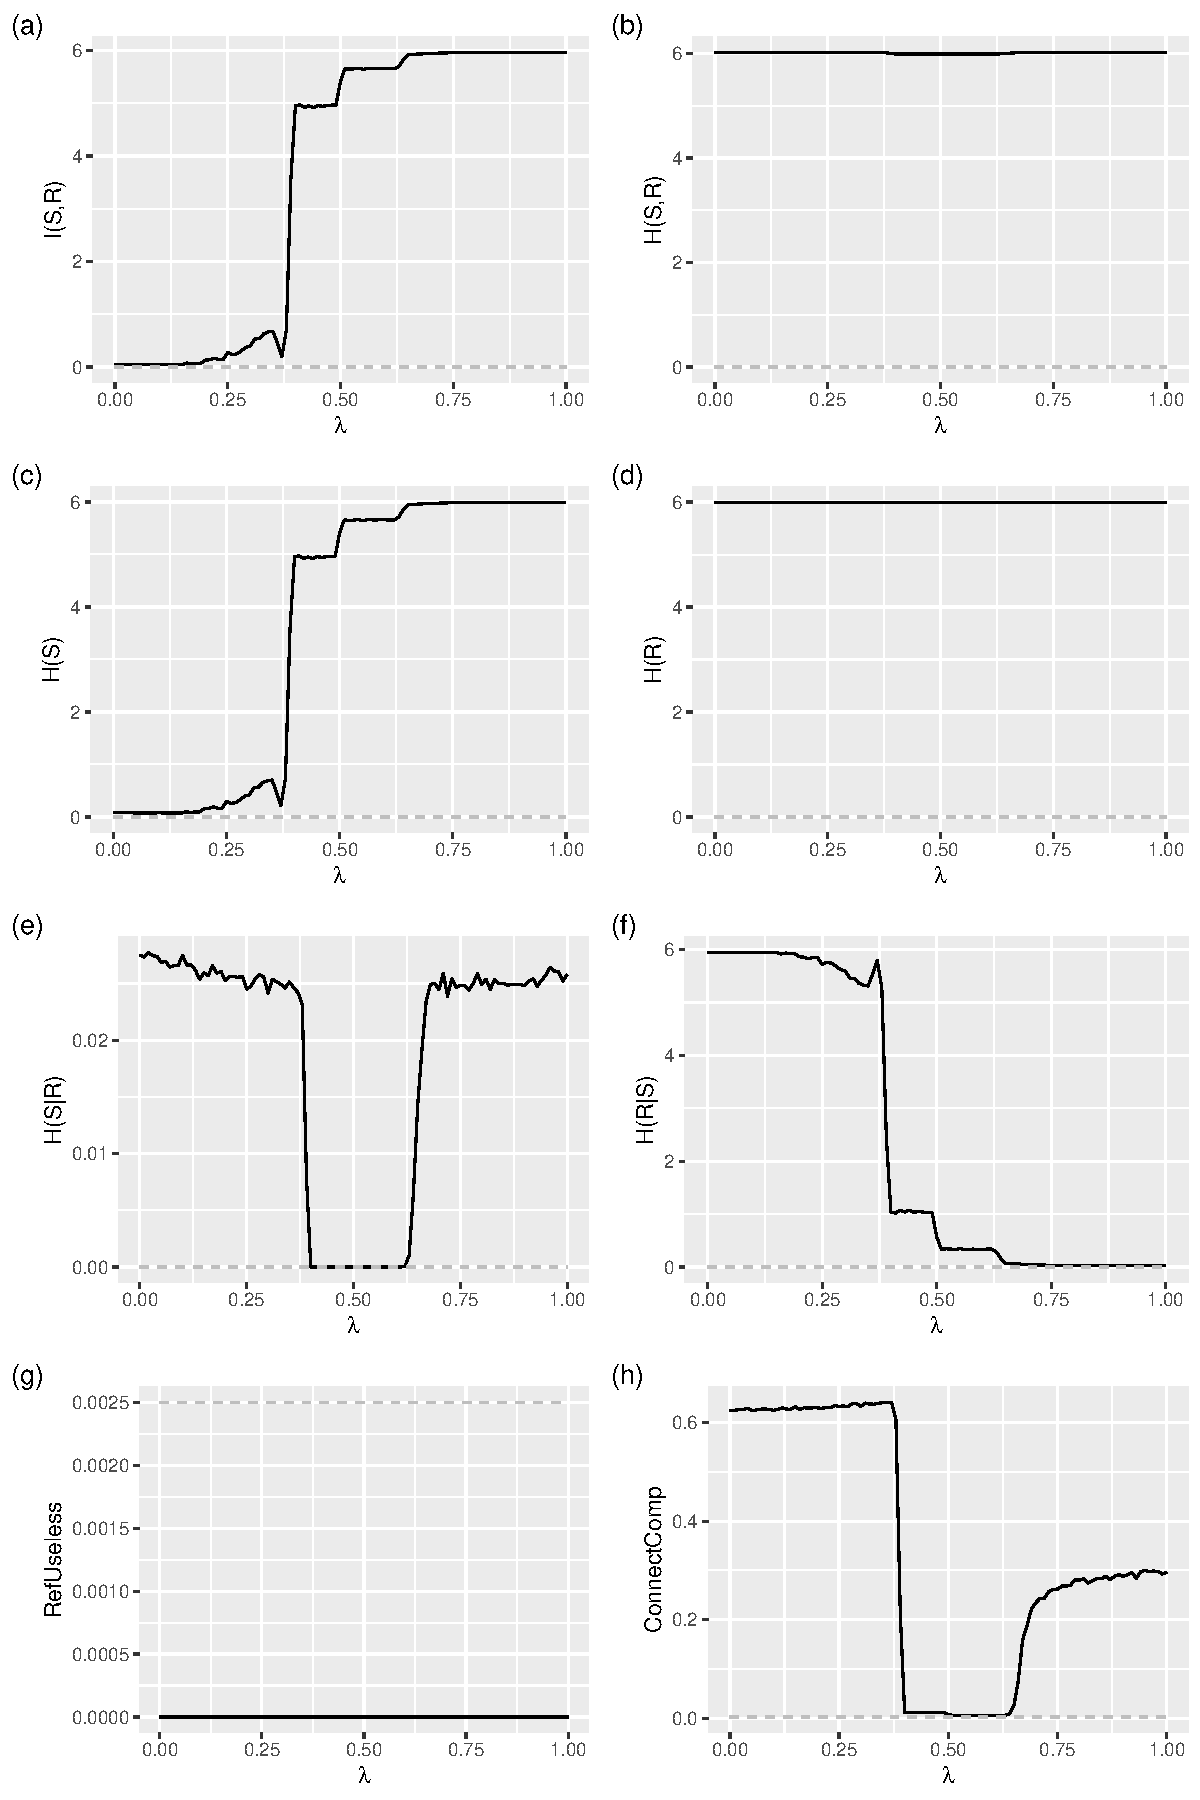
\includegraphics[width=\textwidth]{informationTheoretic_uniform_phi0_nm400_dynamic_singleLink_disallowUnlinked}
  \caption{a}
  \label{fig:informationTheoretic_uniform_phi0_nm400_dynamic_singleLink_disallowUnlinked}
\end{figure}

\begin{figure}
  \centering
  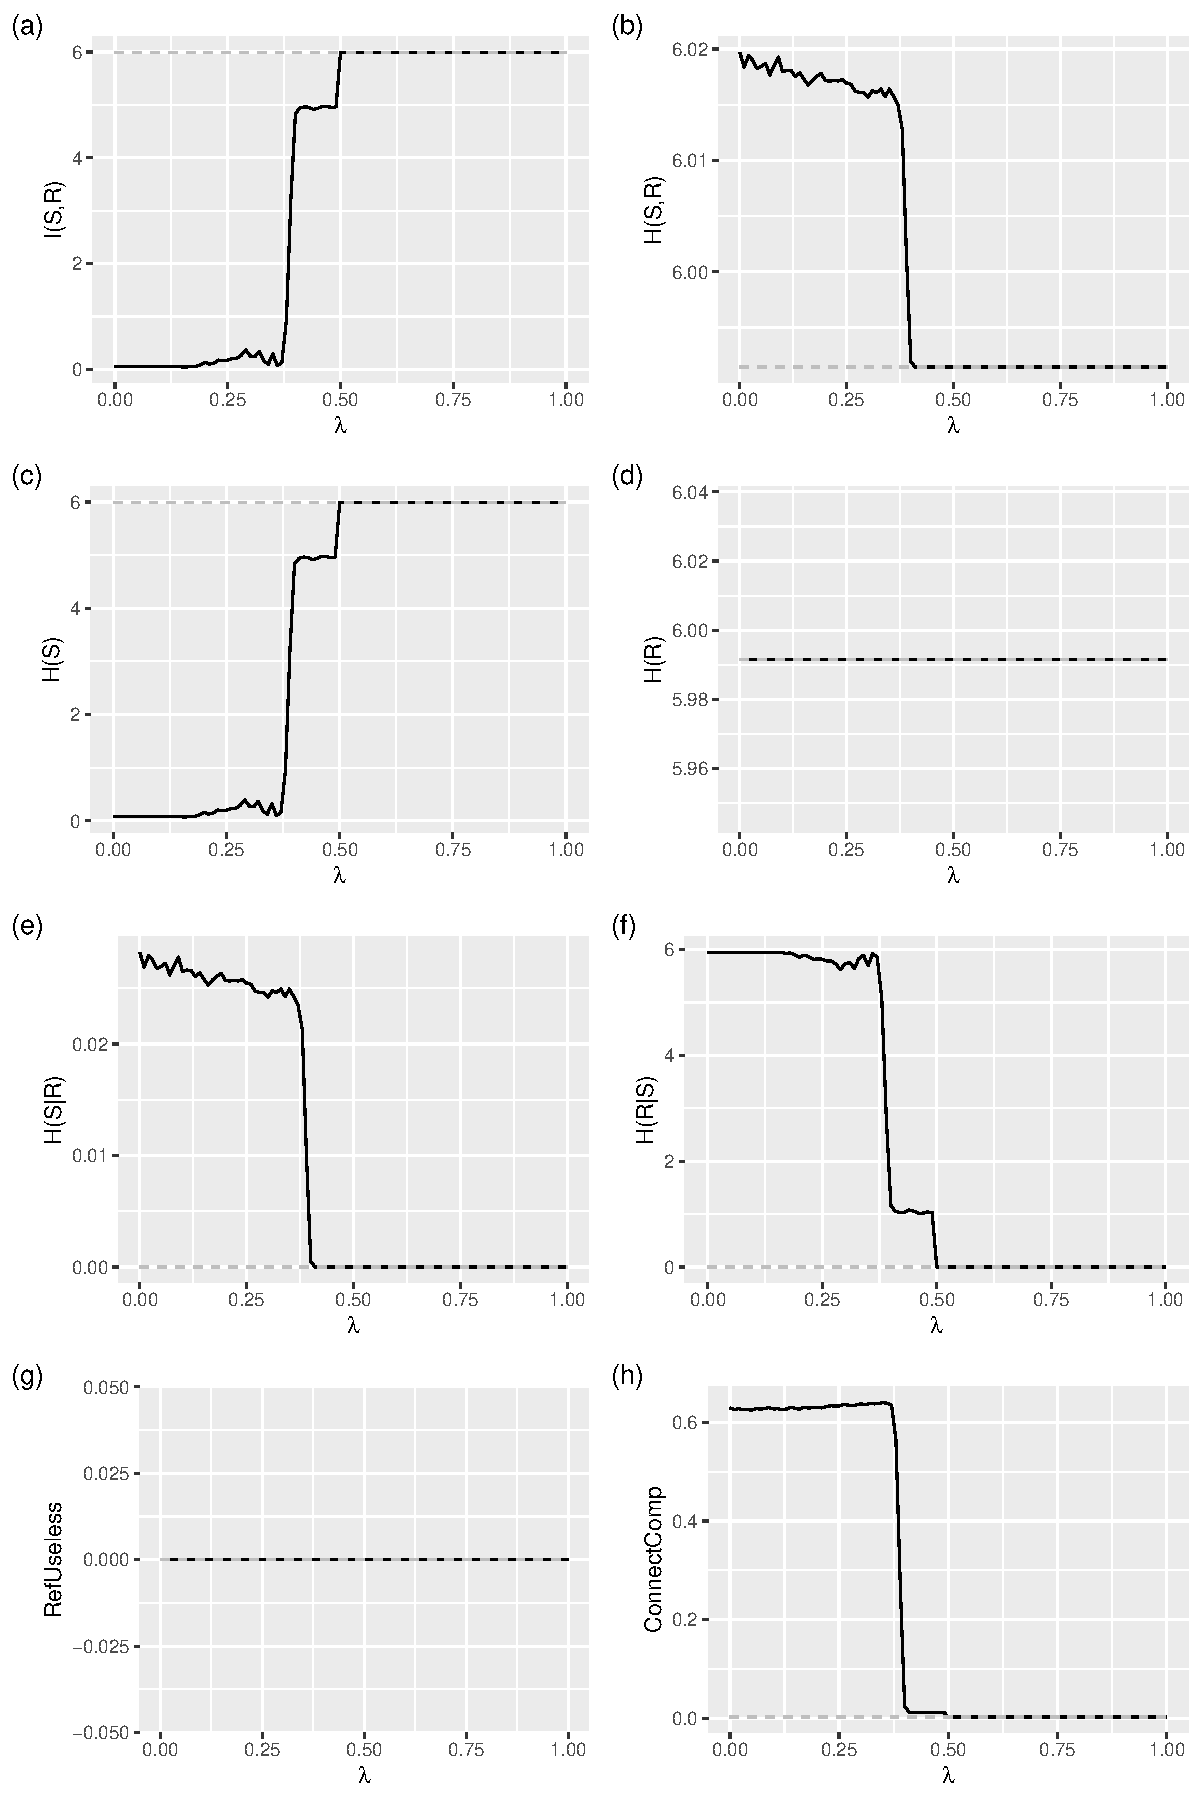
\includegraphics[width=\textwidth]{informationTheoretic_uniform_phi0_nm400_dynamic_oneToOne_disallowUnlinked}
  \caption{a}
  \label{fig:informationTheoretic_uniform_phi0_nm400_dynamic_oneToOne_disallowUnlinked}
\end{figure}

\begin{figure}
  \centering
  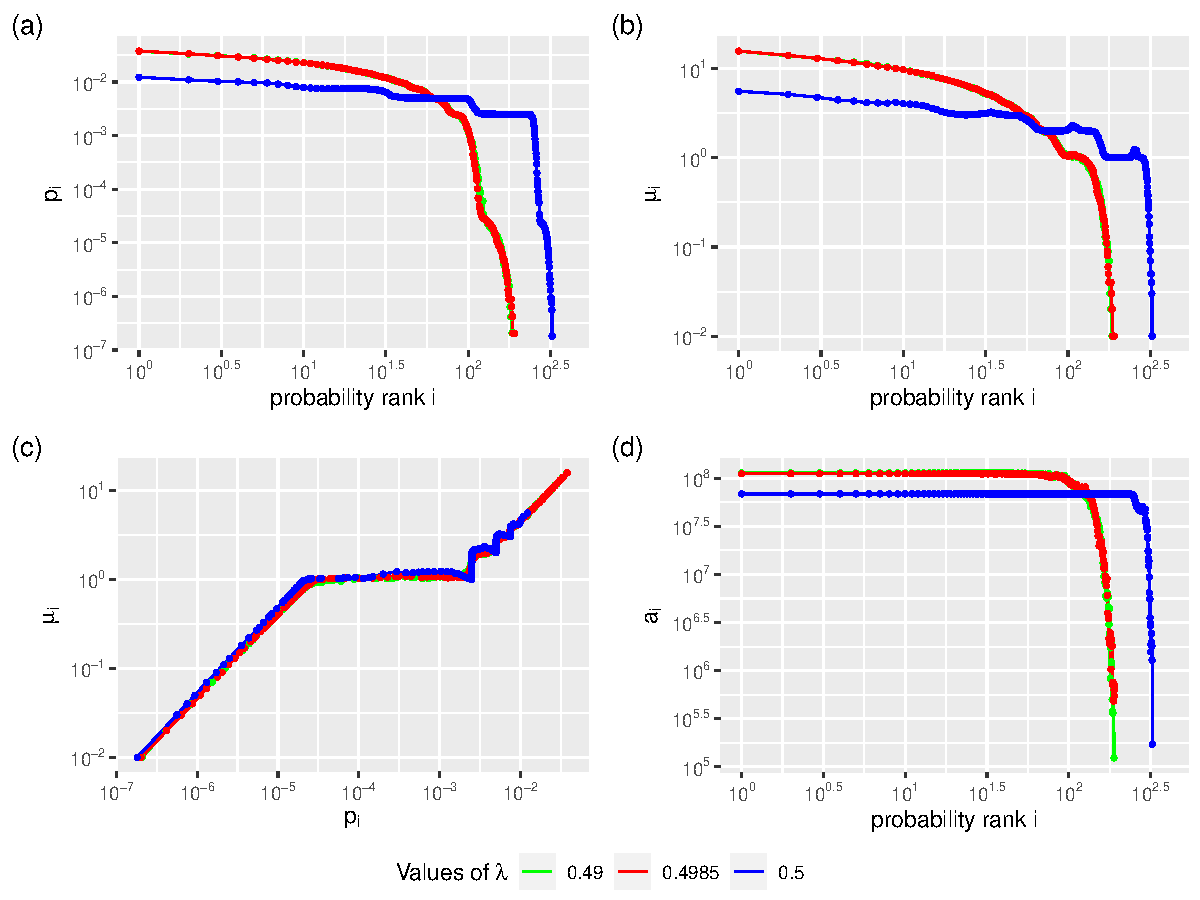
\includegraphics[width=\textwidth,draft]{insideLambda_uniform_phi0_nm400_dynamic_randomBipartite_disallowUnlinked.pdf}
  \caption{a}
  \label{fig:insideLambda_uniform_phi0_nm400_dynamic_randomBipartite_disallowUnlinked}
\end{figure}

\begin{figure}
  \centering
  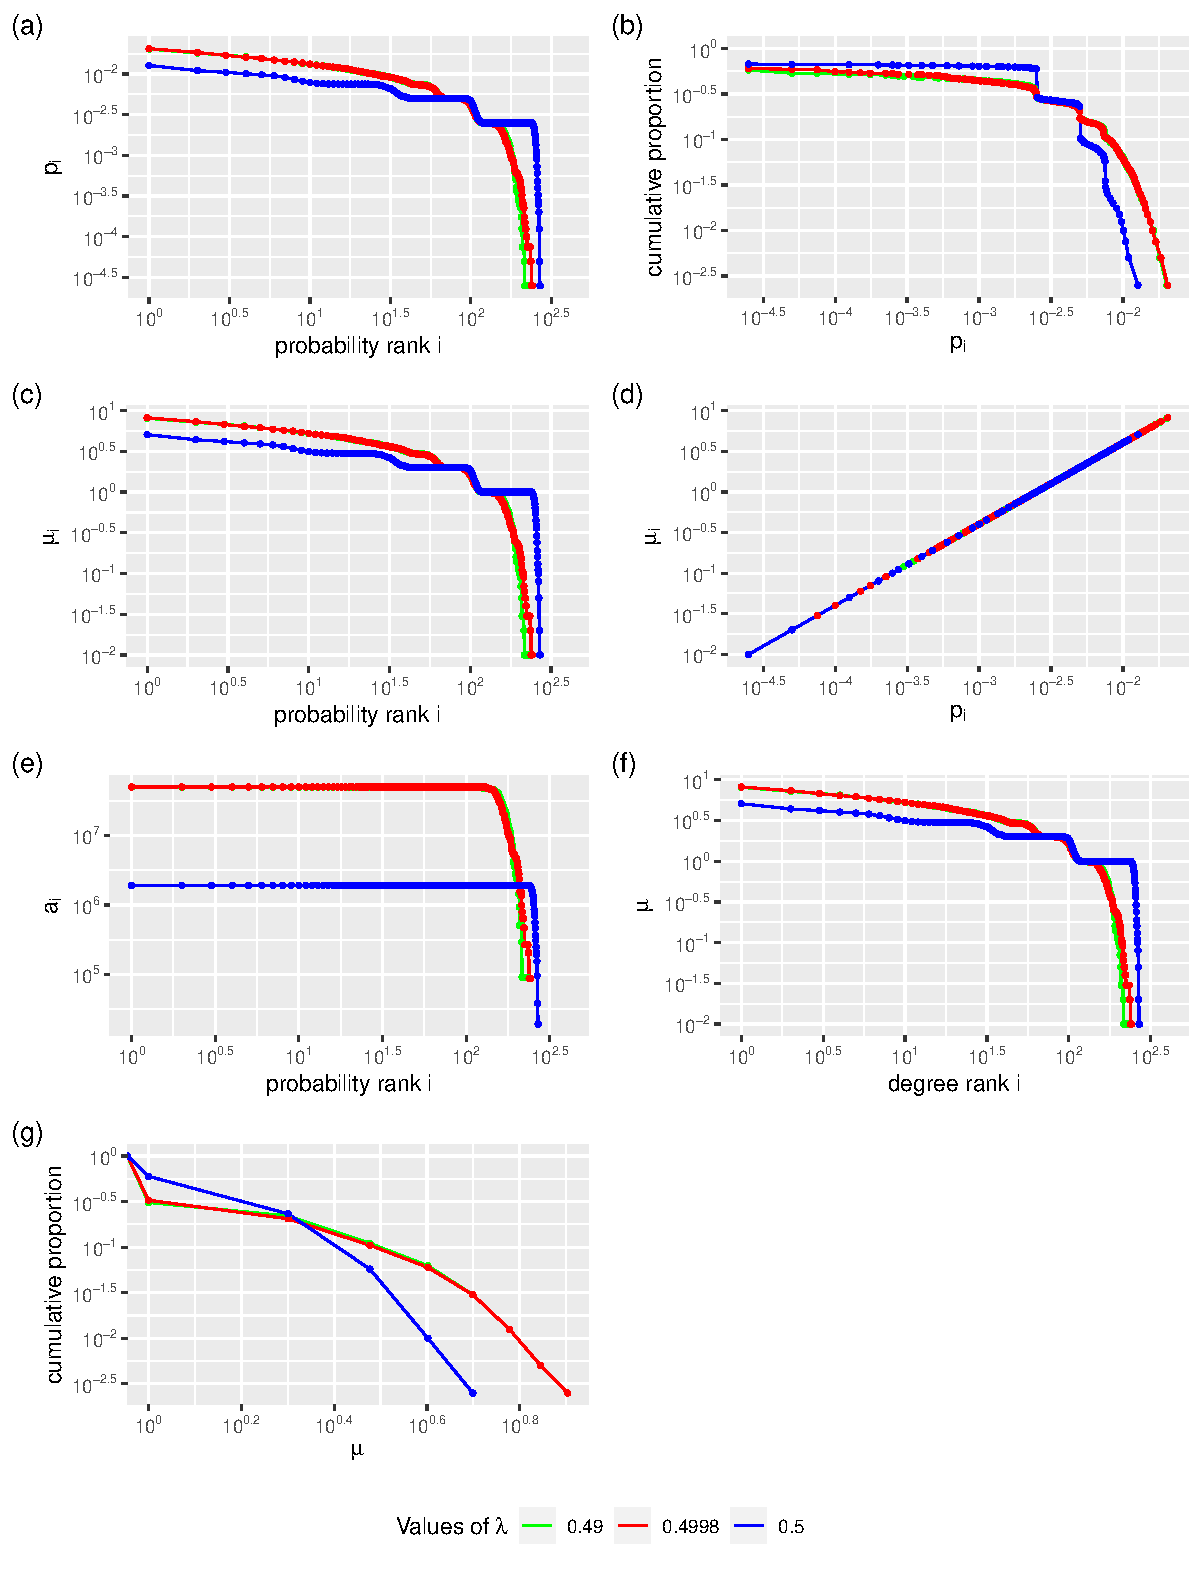
\includegraphics[width=\textwidth,draft]{insideLambda_uniform_phi0_nm400_dynamic_singleLink_disallowUnlinked.pdf}
  \caption{a}
  \label{fig:insideLambda_uniform_phi0_nm400_dynamic_singleLink_disallowUnlinked}
\end{figure}

\begin{figure}
  \centering
  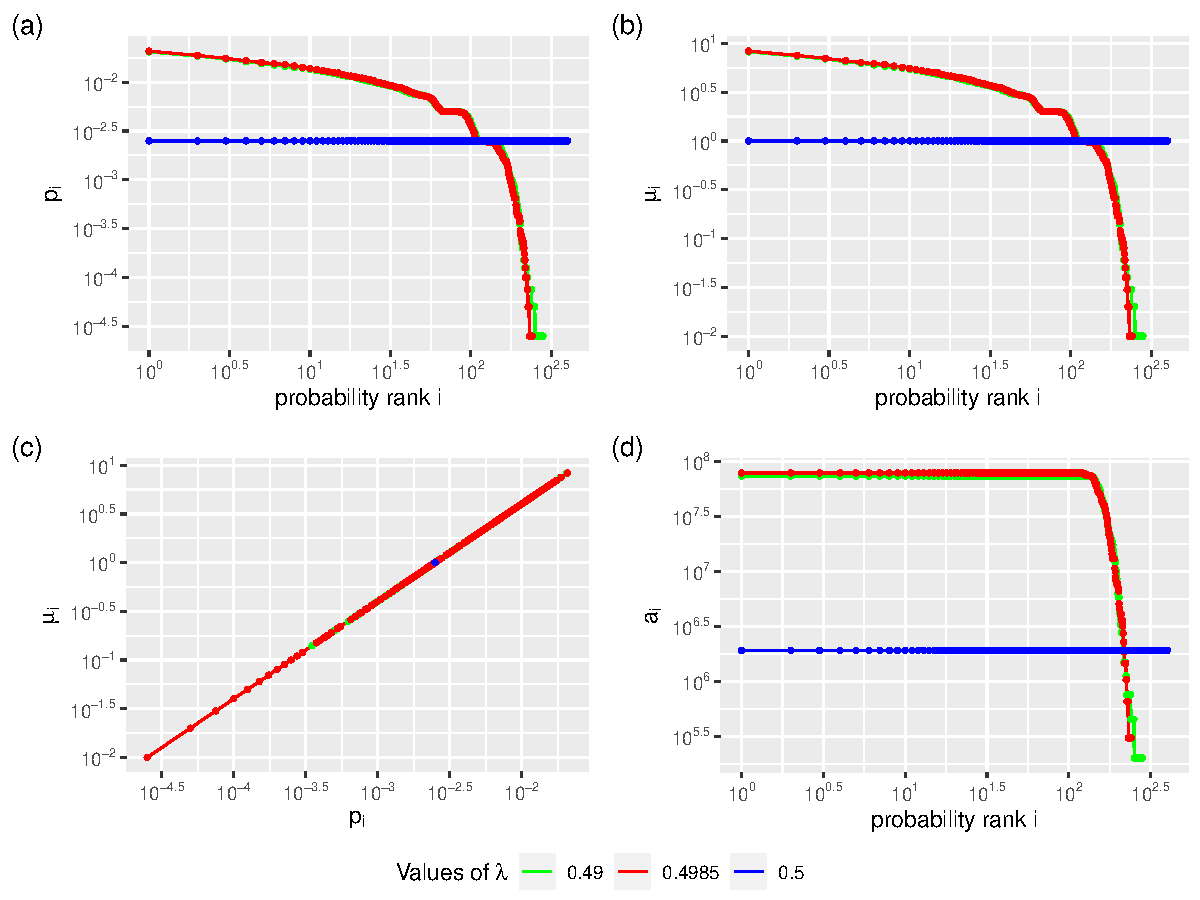
\includegraphics[width=\textwidth,draft]{insideLambda_uniform_phi0_nm400_dynamic_oneToOne_disallowUnlinked.pdf}
  \caption{a}
  \label{fig:insideLambda_uniform_phi0_nm400_dynamic_oneToOne_disallowUnlinked}
\end{figure}

Similar figures have also been generated for $\phi=1$, Figures \ref{fig:informationTheoretic_uniform_phi1_nm400_dynamic_randomBipartite_disallowUnlinked},  \ref{fig:informationTheoretic_uniform_phi1_nm400_dynamic_singleLink_disallowUnlinked} and \ref{fig:informationTheoretic_uniform_phi1_nm400_dynamic_oneToOne_disallowUnlinked} correspond respectively to Figures \ref{fig:informationTheoretic_uniform_phi1_nm400_dynamic_randomBipartite_allowUnlinked},  \ref{fig:informationTheoretic_uniform_phi1_nm400_dynamic_singleLink_allowUnlinked} and \ref{fig:informationTheoretic_uniform_phi1_nm400_dynamic_oneToOne_allowUnlinked}.
Statistical measures for chosen values of $\lambda$ are given in Figures \ref{fig:insideLambda_uniform_phi1_nm400_dynamic_randomBipartite_disallowUnlinked}, \ref{fig:insideLambda_uniform_phi1_nm400_dynamic_singleLink_disallowUnlinked} and \ref{fig:insideLambda_uniform_phi1_nm400_dynamic_oneToOne_disallowUnlinked}.

\begin{figure}
  \centering
  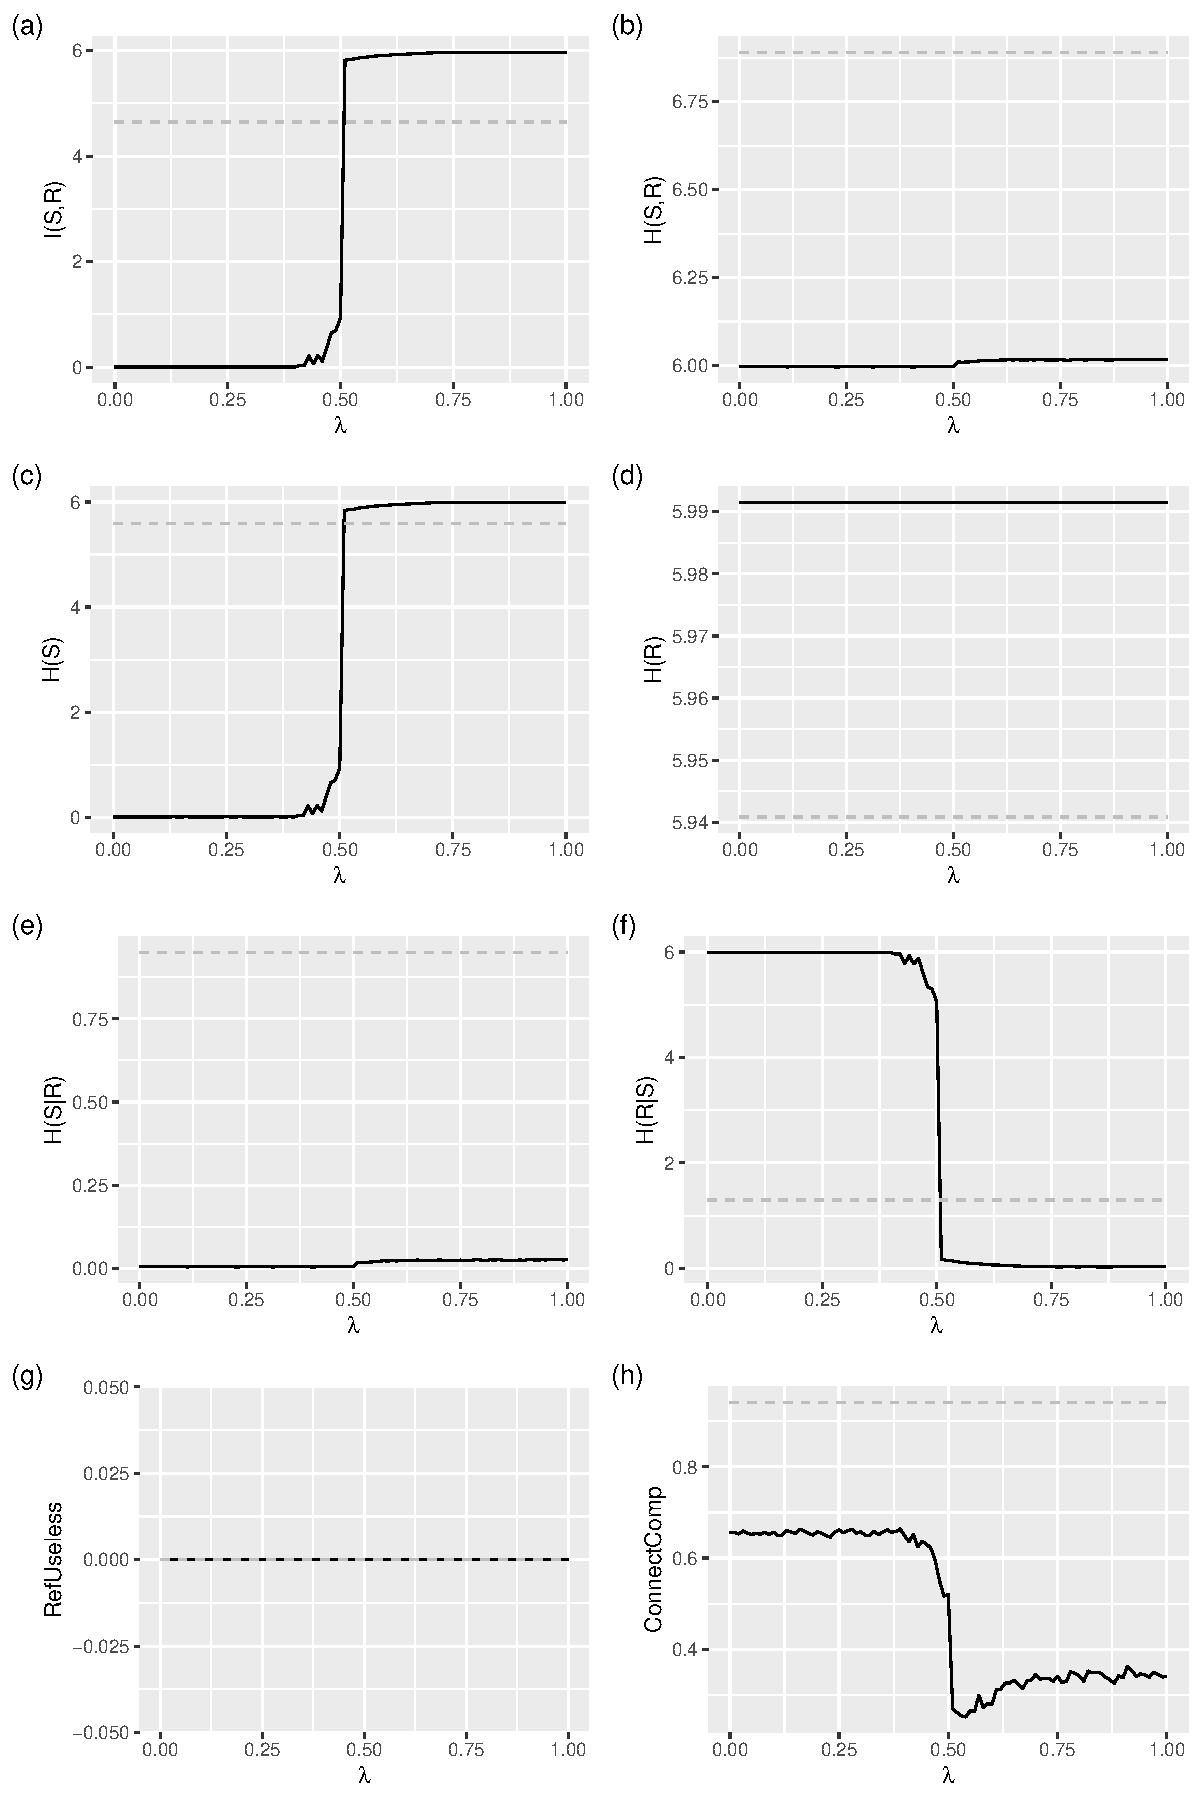
\includegraphics[width=\textwidth]{informationTheoretic_uniform_phi1_nm400_dynamic_randomBipartite_disallowUnlinked}
  \caption{a}
  \label{fig:informationTheoretic_uniform_phi1_nm400_dynamic_randomBipartite_disallowUnlinked}
\end{figure}

\begin{figure}
  \centering
  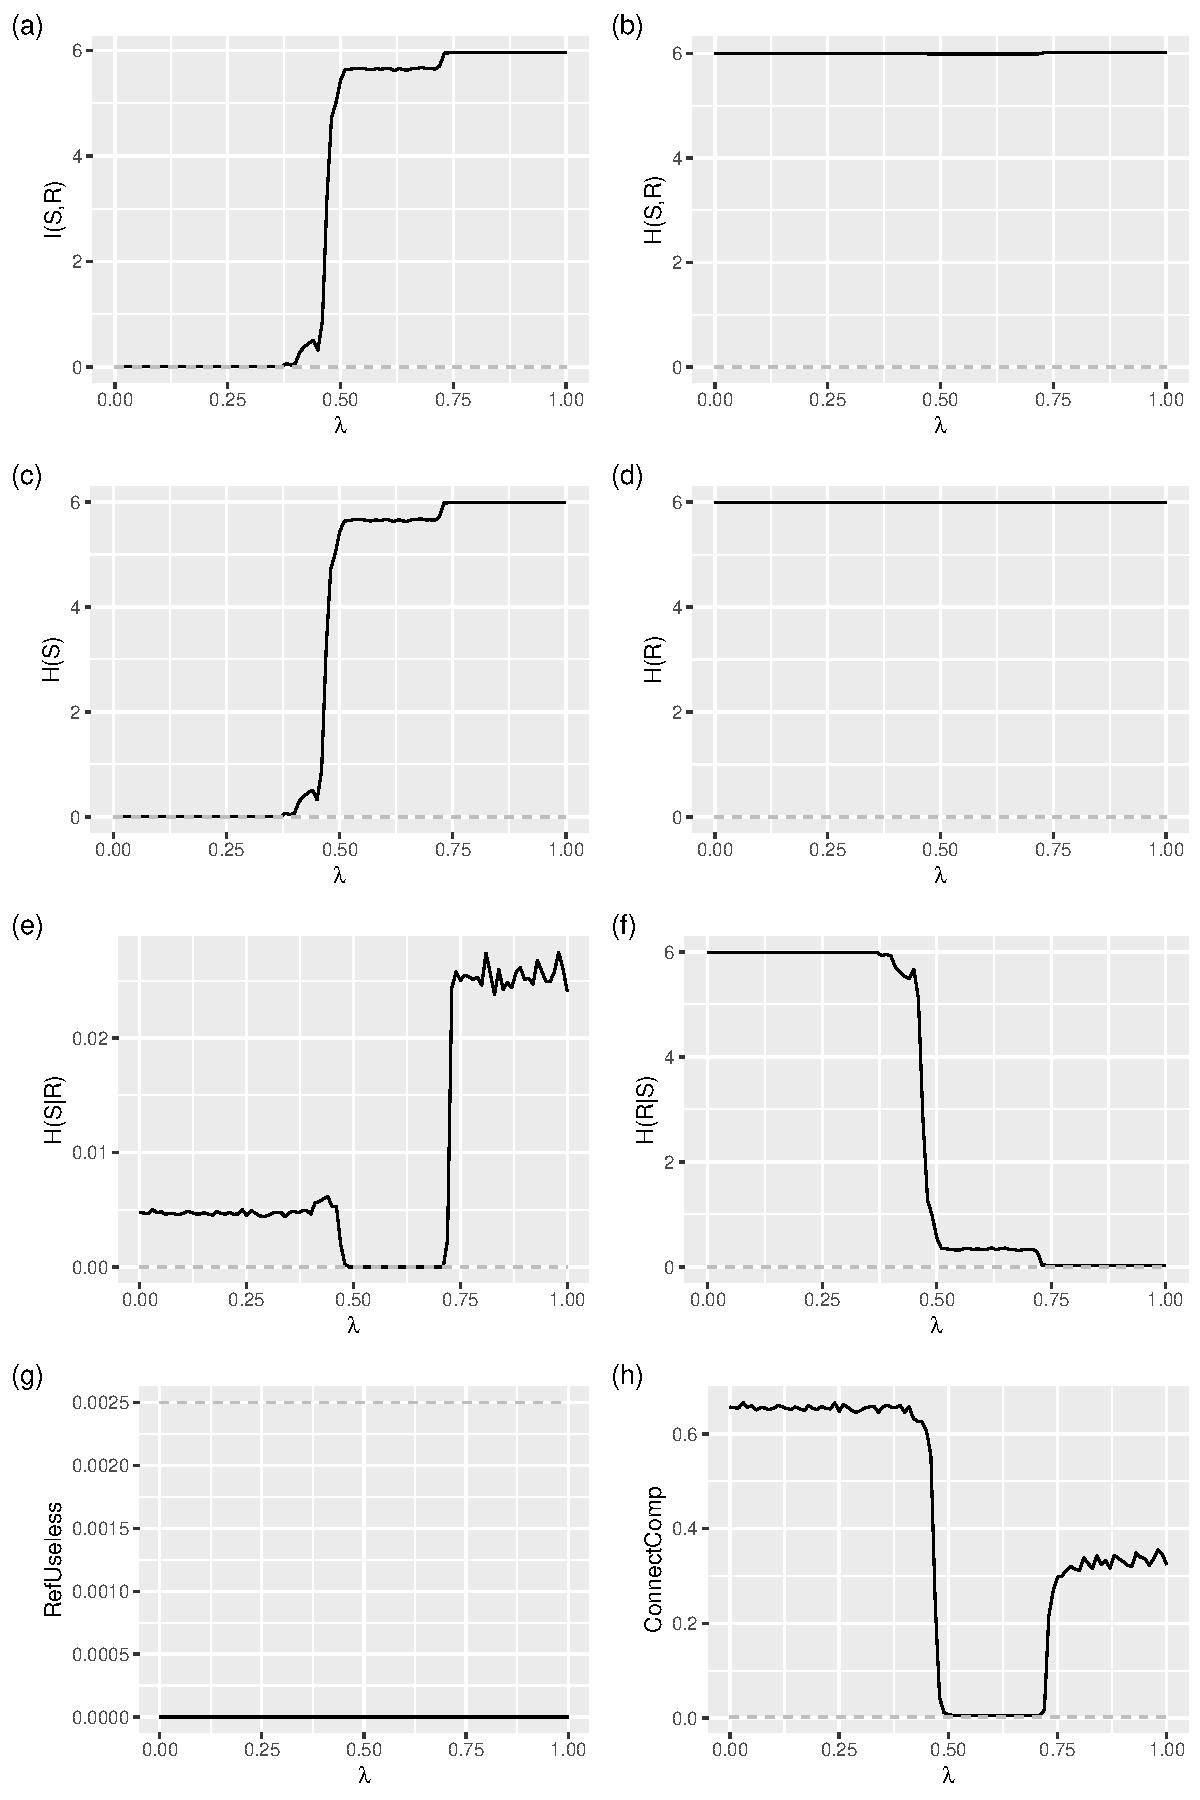
\includegraphics[width=\textwidth]{informationTheoretic_uniform_phi1_nm400_dynamic_singleLink_disallowUnlinked}
  \caption{a}
  \label{fig:informationTheoretic_uniform_phi1_nm400_dynamic_singleLink_disallowUnlinked}
\end{figure}

\begin{figure}
  \centering
  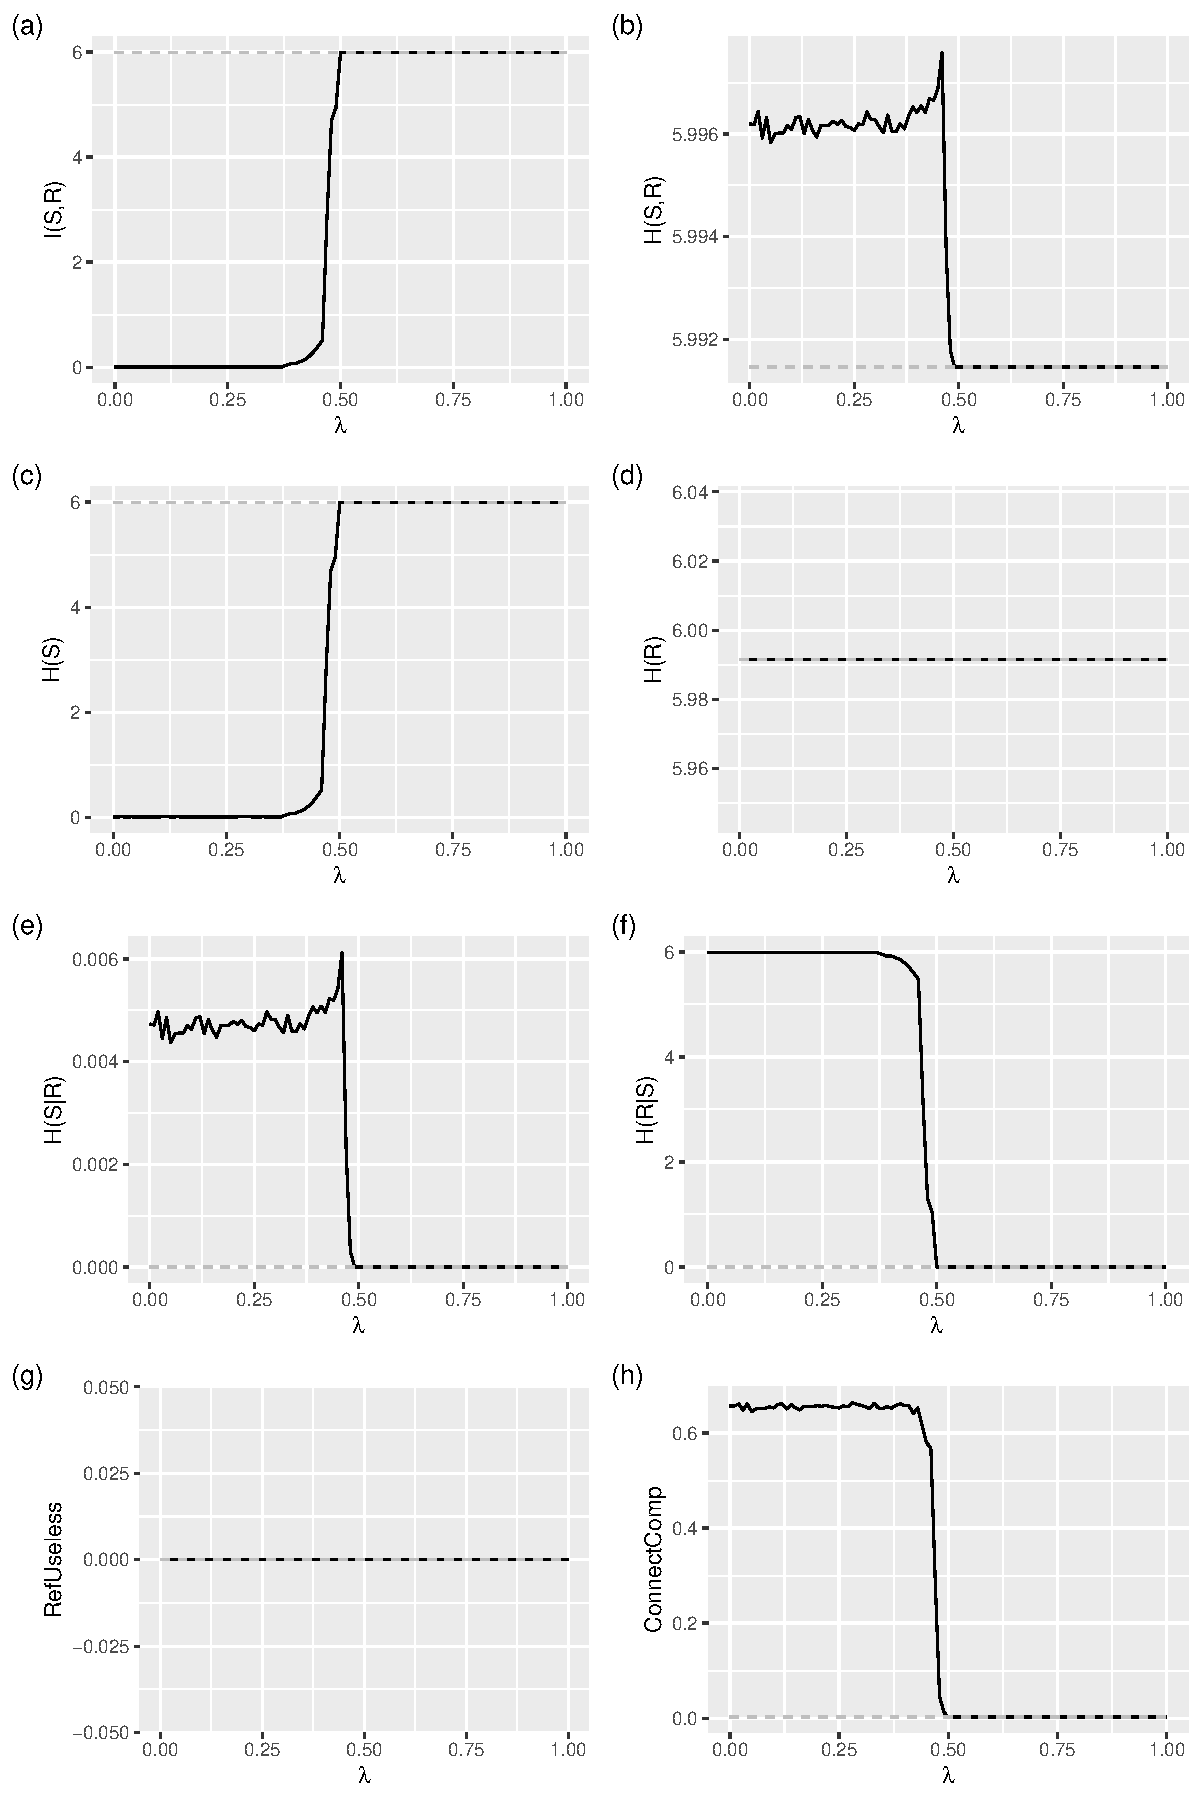
\includegraphics[width=\textwidth]{informationTheoretic_uniform_phi1_nm400_dynamic_oneToOne_disallowUnlinked}
  \caption{this happens for $\phi=1$ but not for $\phi=0$}
  \label{fig:informationTheoretic_uniform_phi1_nm400_dynamic_oneToOne_disallowUnlinked}
\end{figure}

\begin{figure}
  \centering
  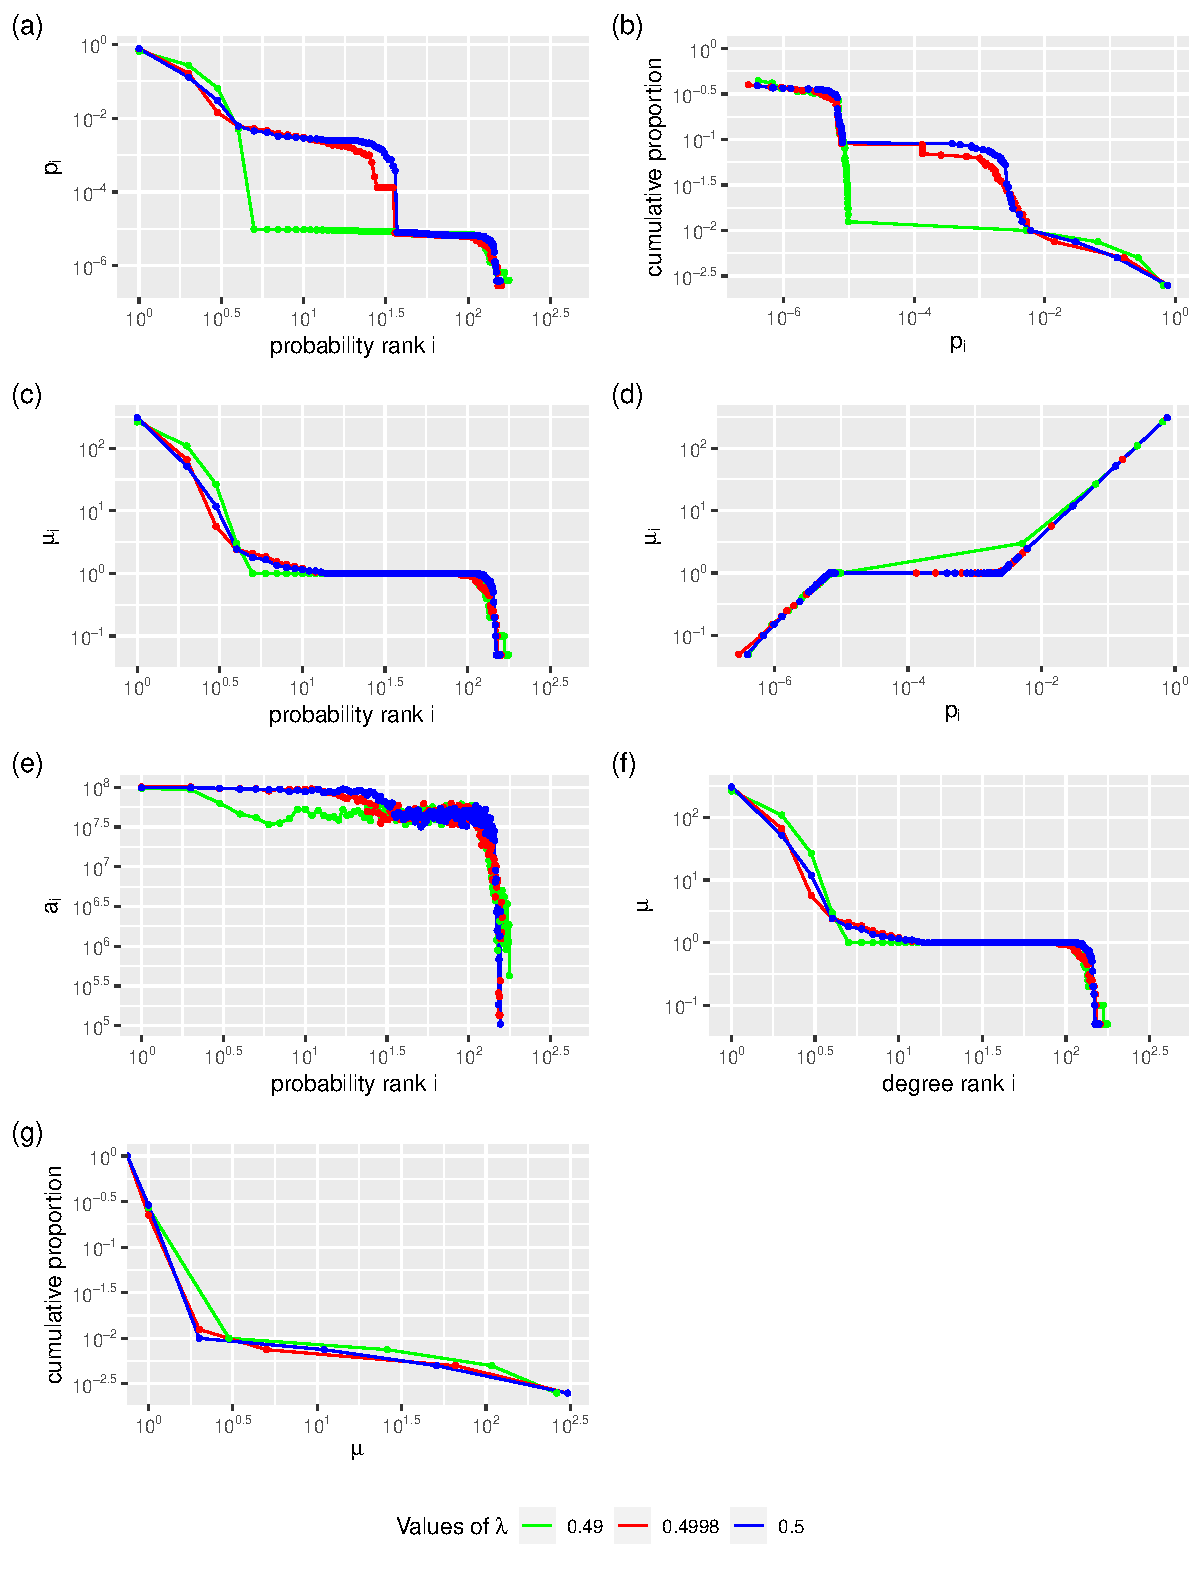
\includegraphics[width=\textwidth,draft]{insideLambda_uniform_phi1_nm400_dynamic_randomBipartite_disallowUnlinked.pdf}
  \caption{a}
  \label{fig:insideLambda_uniform_phi1_nm400_dynamic_randomBipartite_disallowUnlinked}
\end{figure}

\begin{figure}
  \centering
  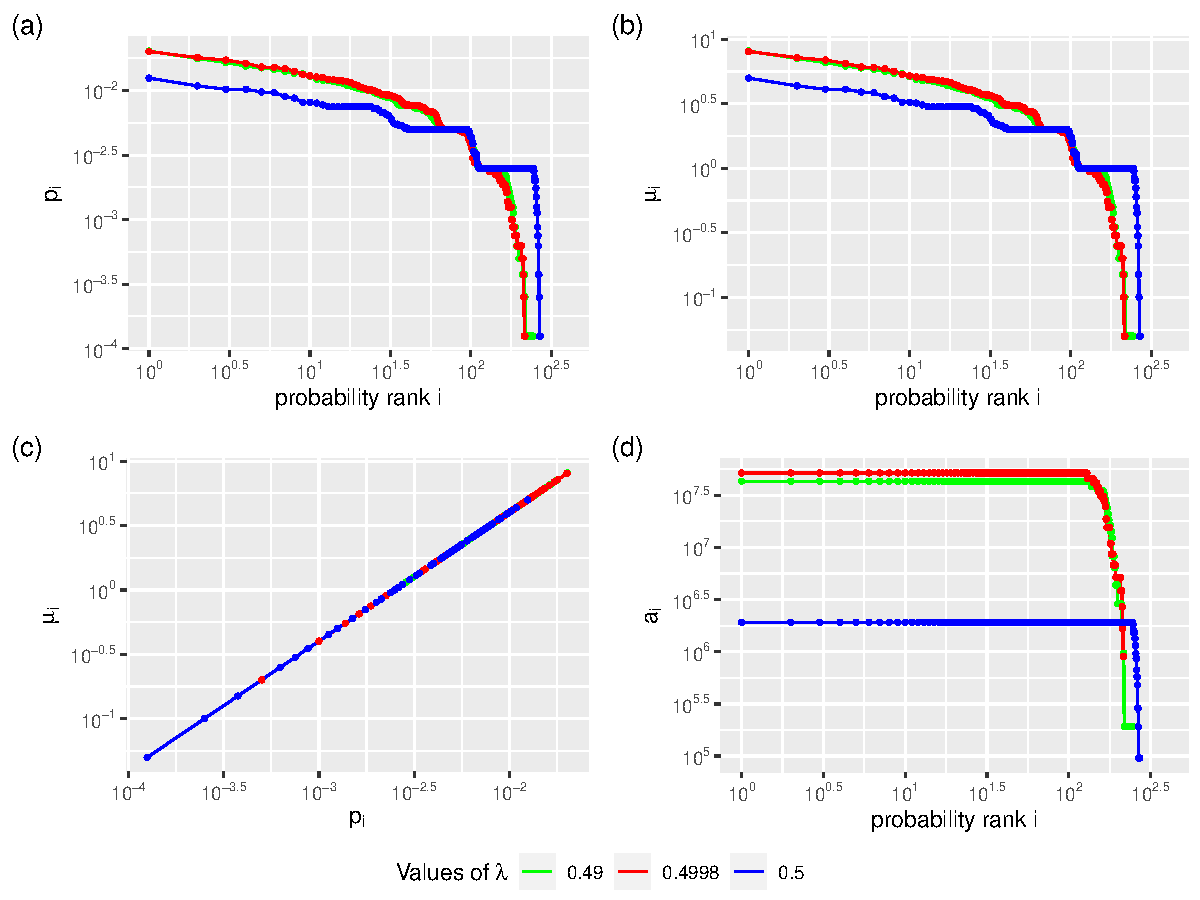
\includegraphics[width=\textwidth,draft]{insideLambda_uniform_phi1_nm400_dynamic_singleLink_disallowUnlinked.pdf}
  \caption{a}
  \label{fig:insideLambda_uniform_phi1_nm400_dynamic_singleLink_disallowUnlinked}
\end{figure}

\begin{figure}
  \centering
  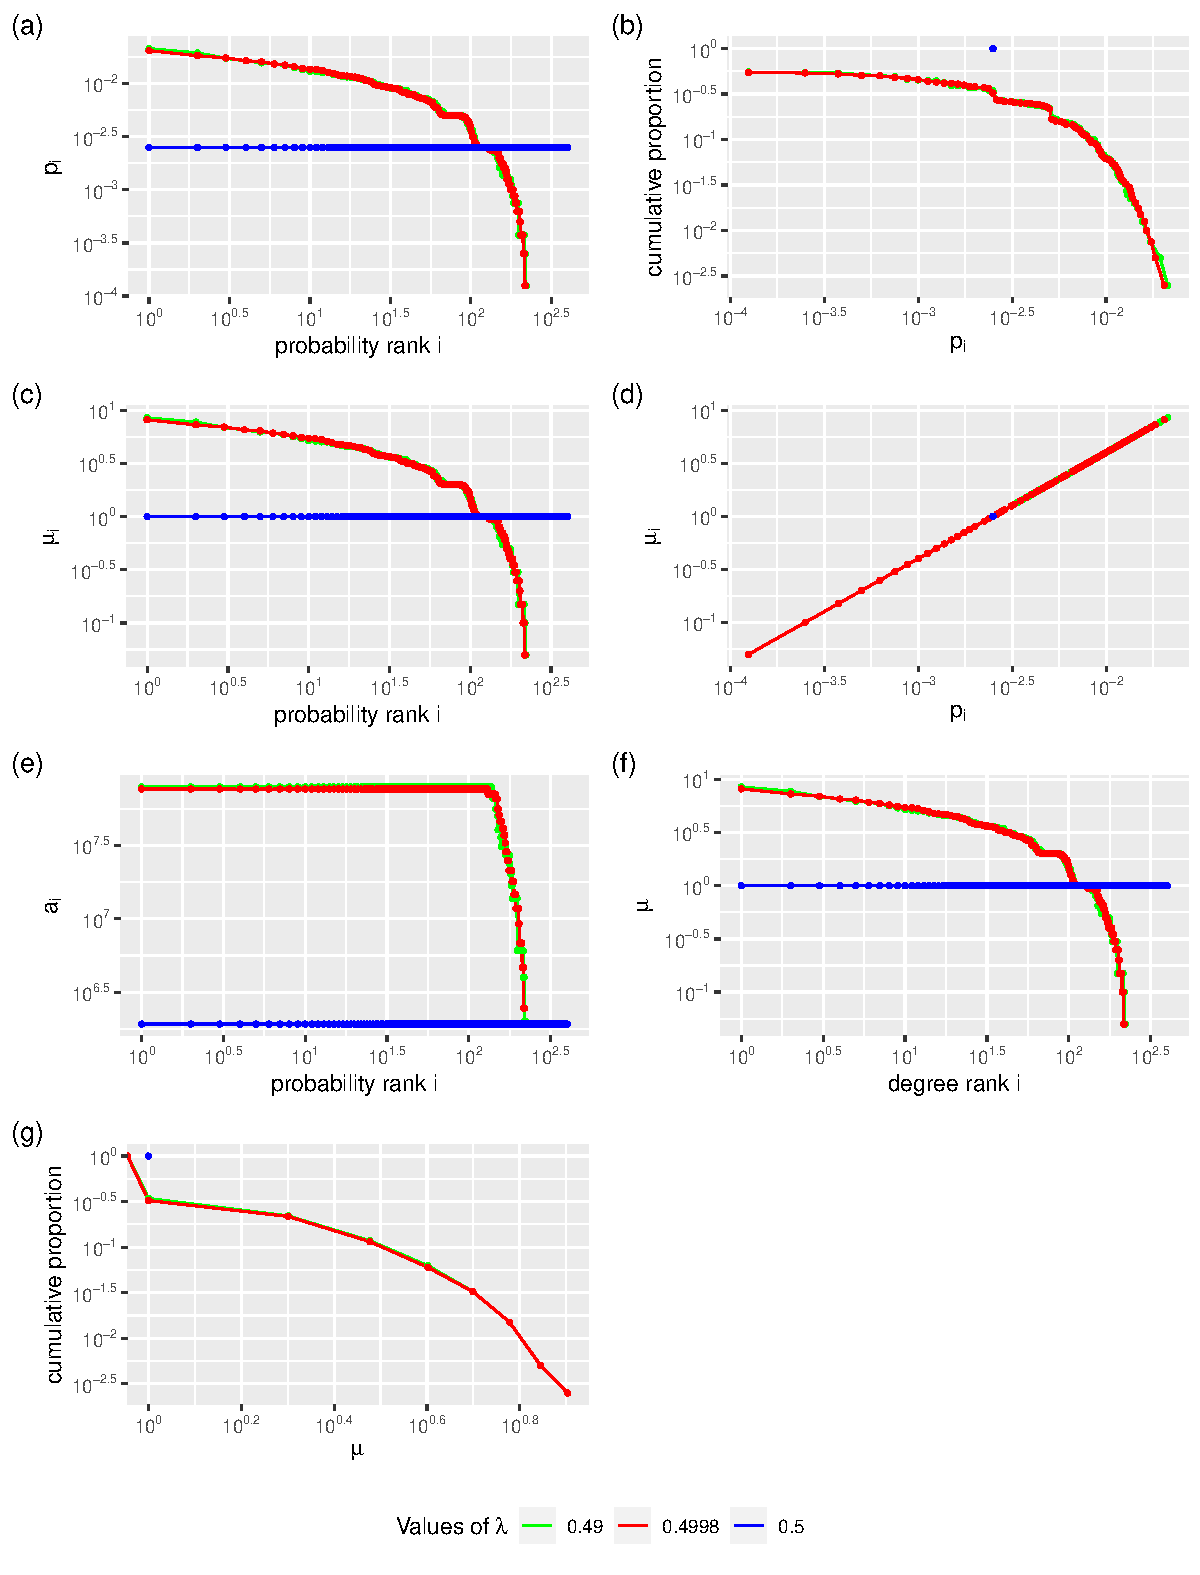
\includegraphics[width=\textwidth,draft]{insideLambda_uniform_phi1_nm400_dynamic_oneToOne_disallowUnlinked.pdf}
  \caption{a}
  \label{fig:insideLambda_uniform_phi1_nm400_dynamic_oneToOne_disallowUnlinked}
\end{figure}

%%% Local Variables:
%%% mode: latex
%%% TeX-master: "tfm"
%%% End:
